\documentclass[a4paper, ngerman, 12pt,parskip=half]{scrreprt}
\usepackage{babel} % für Silbentrennung, eingedeutschte Verzeichnisnamen, etc.
\usepackage[utf8]{inputenc} % UTF8 Encoding
\usepackage[T1]{fontenc}  % Lateinisches Alphabet (T2 für Russisch, etc.)
\usepackage{booktabs} % für schöne Tabellen, siehe Termin 1
\usepackage{blindtext}
\usepackage{graphicx}
\usepackage{microtype} % Mikrotypografie, mit optischem Randausgleich
\usepackage{subcaption}

%\usepackage{palatino} % Palatino Schrift
\usepackage{iwona} % iwona Schrift

\usepackage[headsepline=0.5pt,footsepline=1pt]{scrlayer-scrpage}
\KOMAoptions{headwidth=1.1\textwidth,footwidth=1.1\textwidth}
\pagestyle{scrheadings}
\clearpairofpagestyles

\automark{section}
\ohead[\headmark]{\headmark}
\ofoot[\pagemark]{\pagemark}
\ifoot[ifoot1]{ifoot2} % inner foot
\ihead[ihead1]{ihead2} % inner head
\cfoot[cfoot1]{cfoot2} % center foot
\chead[chead1]{chead2} % center head

\begin{document}

\begin{titlepage}
{\large\textbf{Fernuni Hagen \\ 12345 Hagen \\ Lehrstuhl für Angew. Wissenschaften}}

\vspace*{4cm}

{\bfseries\huge Python und Perl im Vergleich -- Warum Python immer gewinnt! }

\begin{center}
	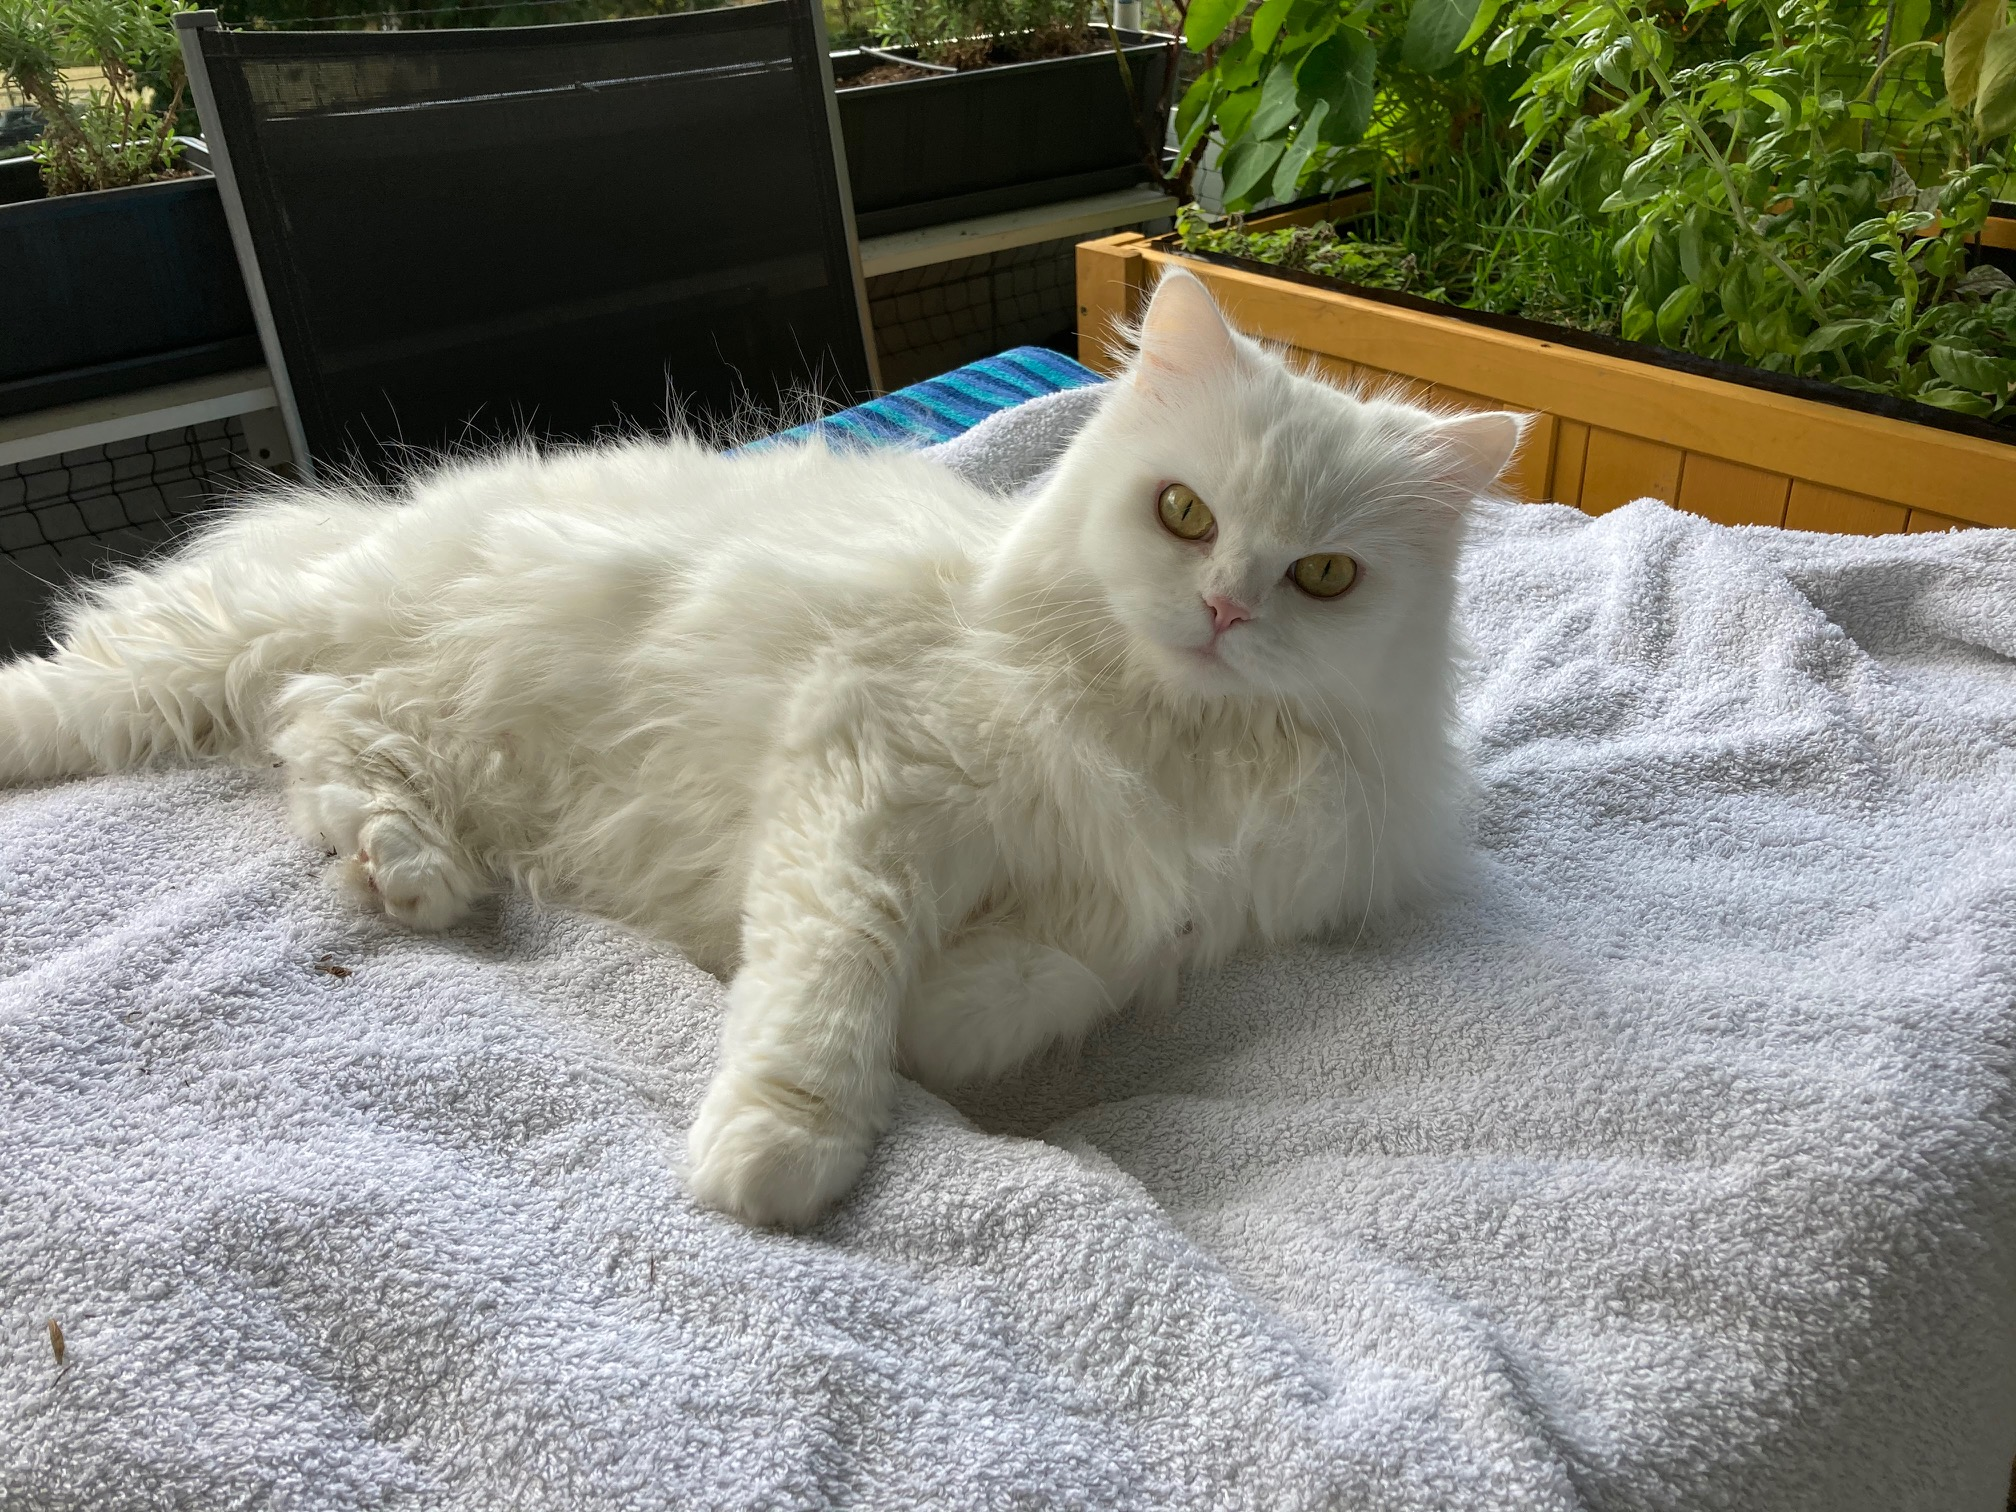
\includegraphics[width=0.2\textwidth]{Bilder/Katze1}
\end{center}

\vfill
Uwe Ziegenhagen \\
Matrikelnummer 31415927 \\
Köln, den \today 
\end{titlepage}

\tableofcontents
\listoffigures
\listoftables
	
\chapter{Einführung in das Thema}	
\section{Literaturüberblick}

In diesem Abschnitt wollen wir kurz die aktuelle Literatur zum Thema besprechen.	
	
\blindtext[10]

\begin{figure}
	\centering
	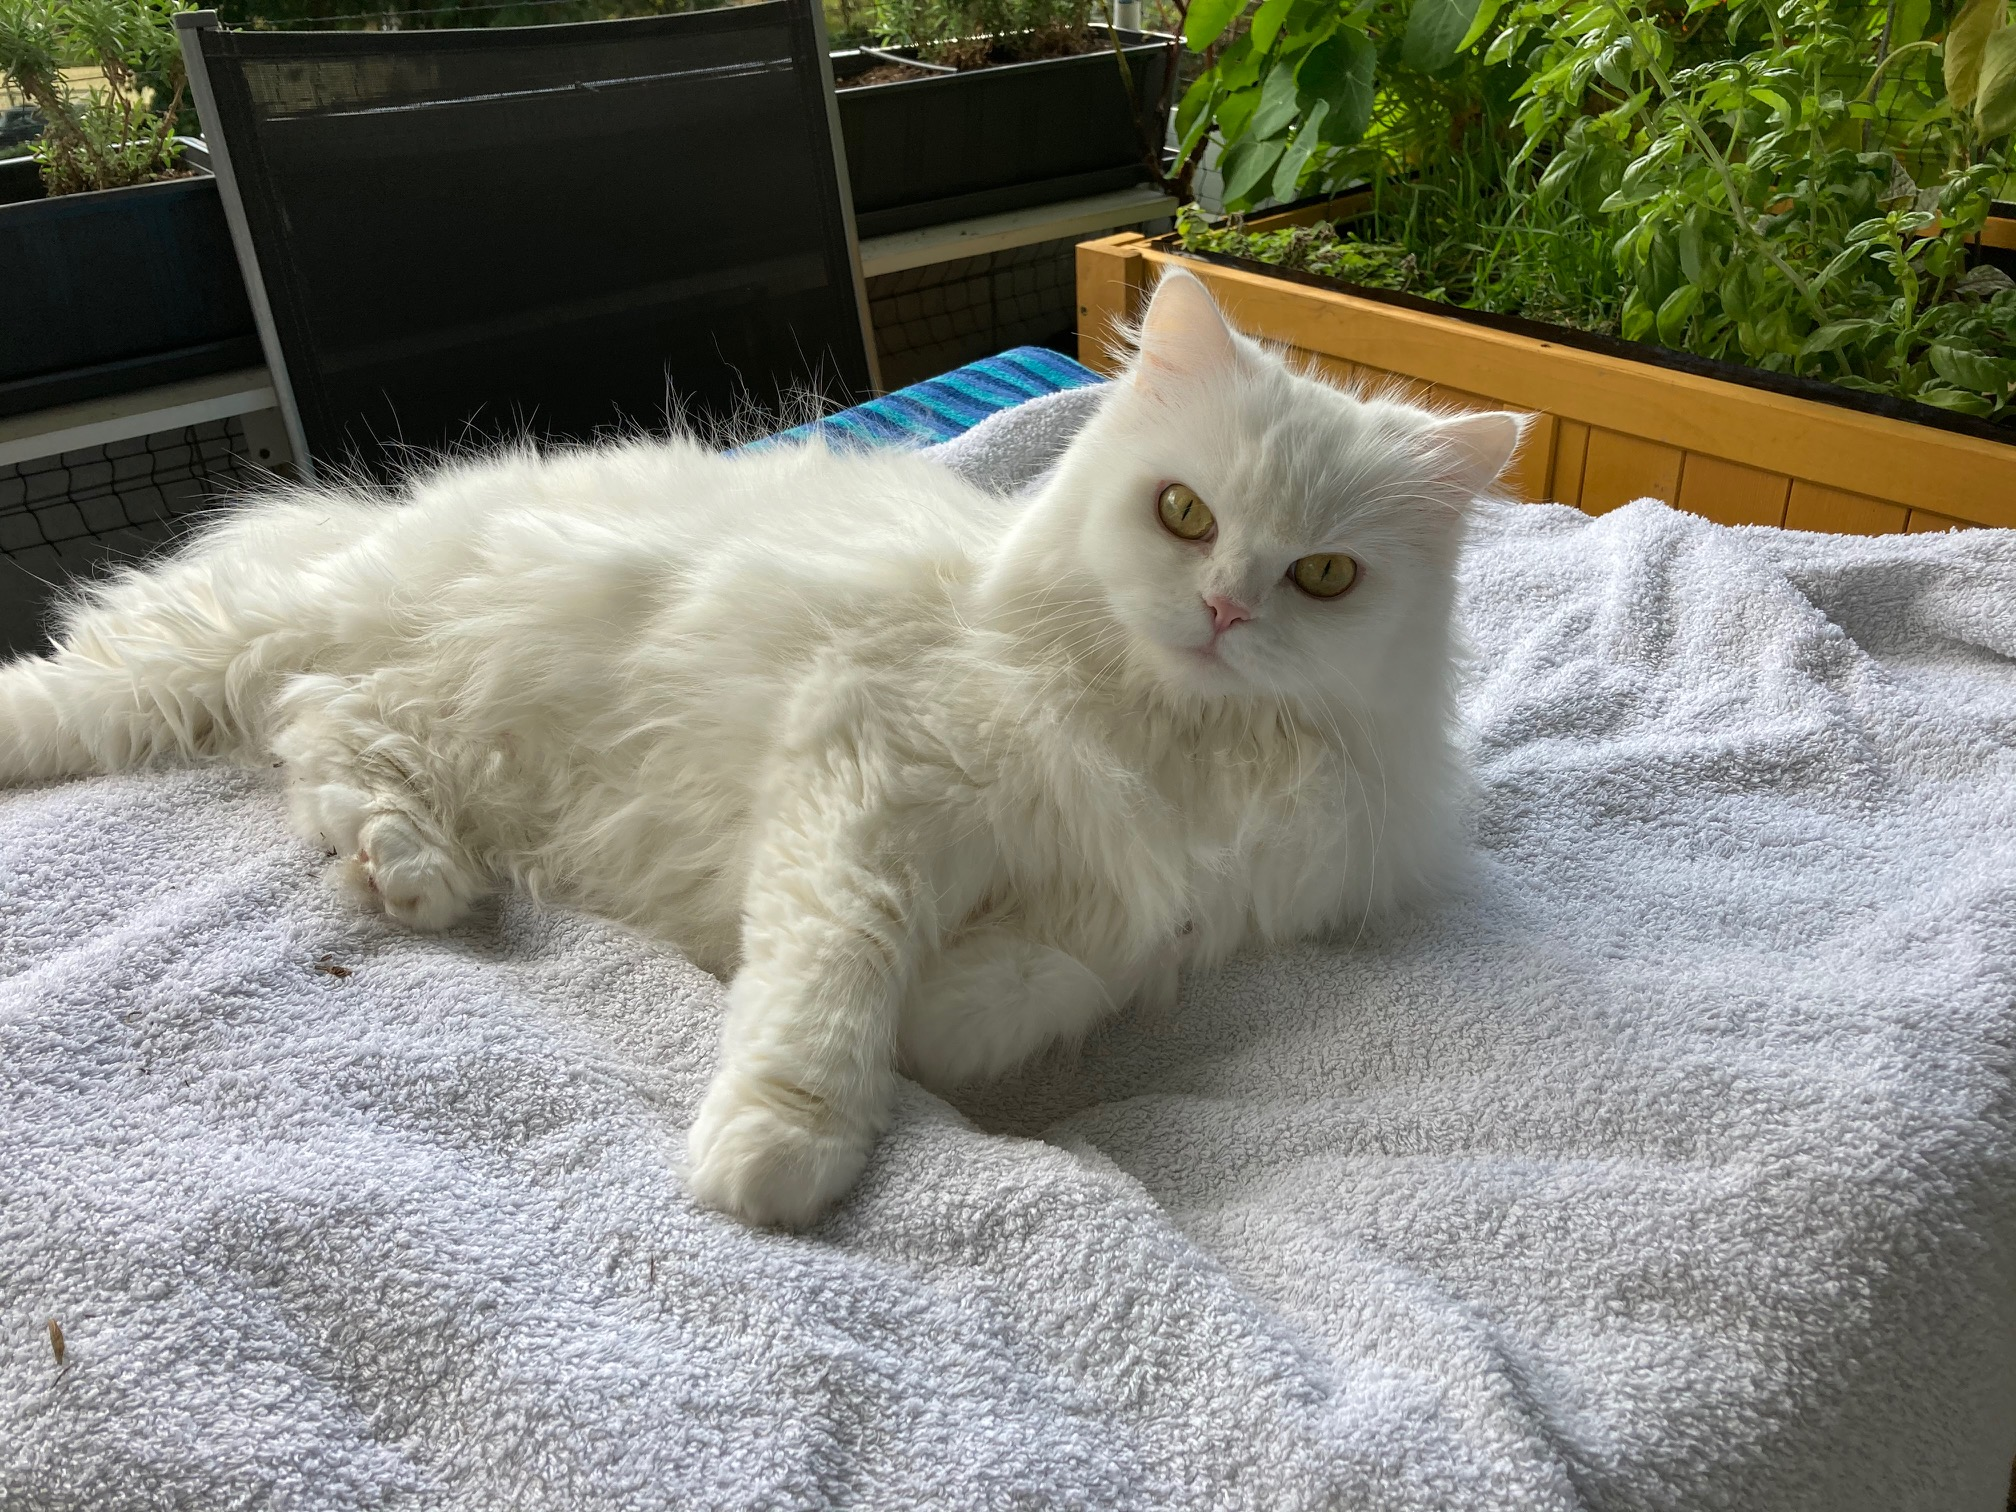
\includegraphics[width=0.75\textwidth]{Bilder/Katze1}
	\caption{Eine Miezekatze}\label{fig:katze1}
\end{figure}

\blindtext[10]

\begin{figure}
	\centering
	\subcaptionbox{Eine Katze \label{fig:cat1}}
	{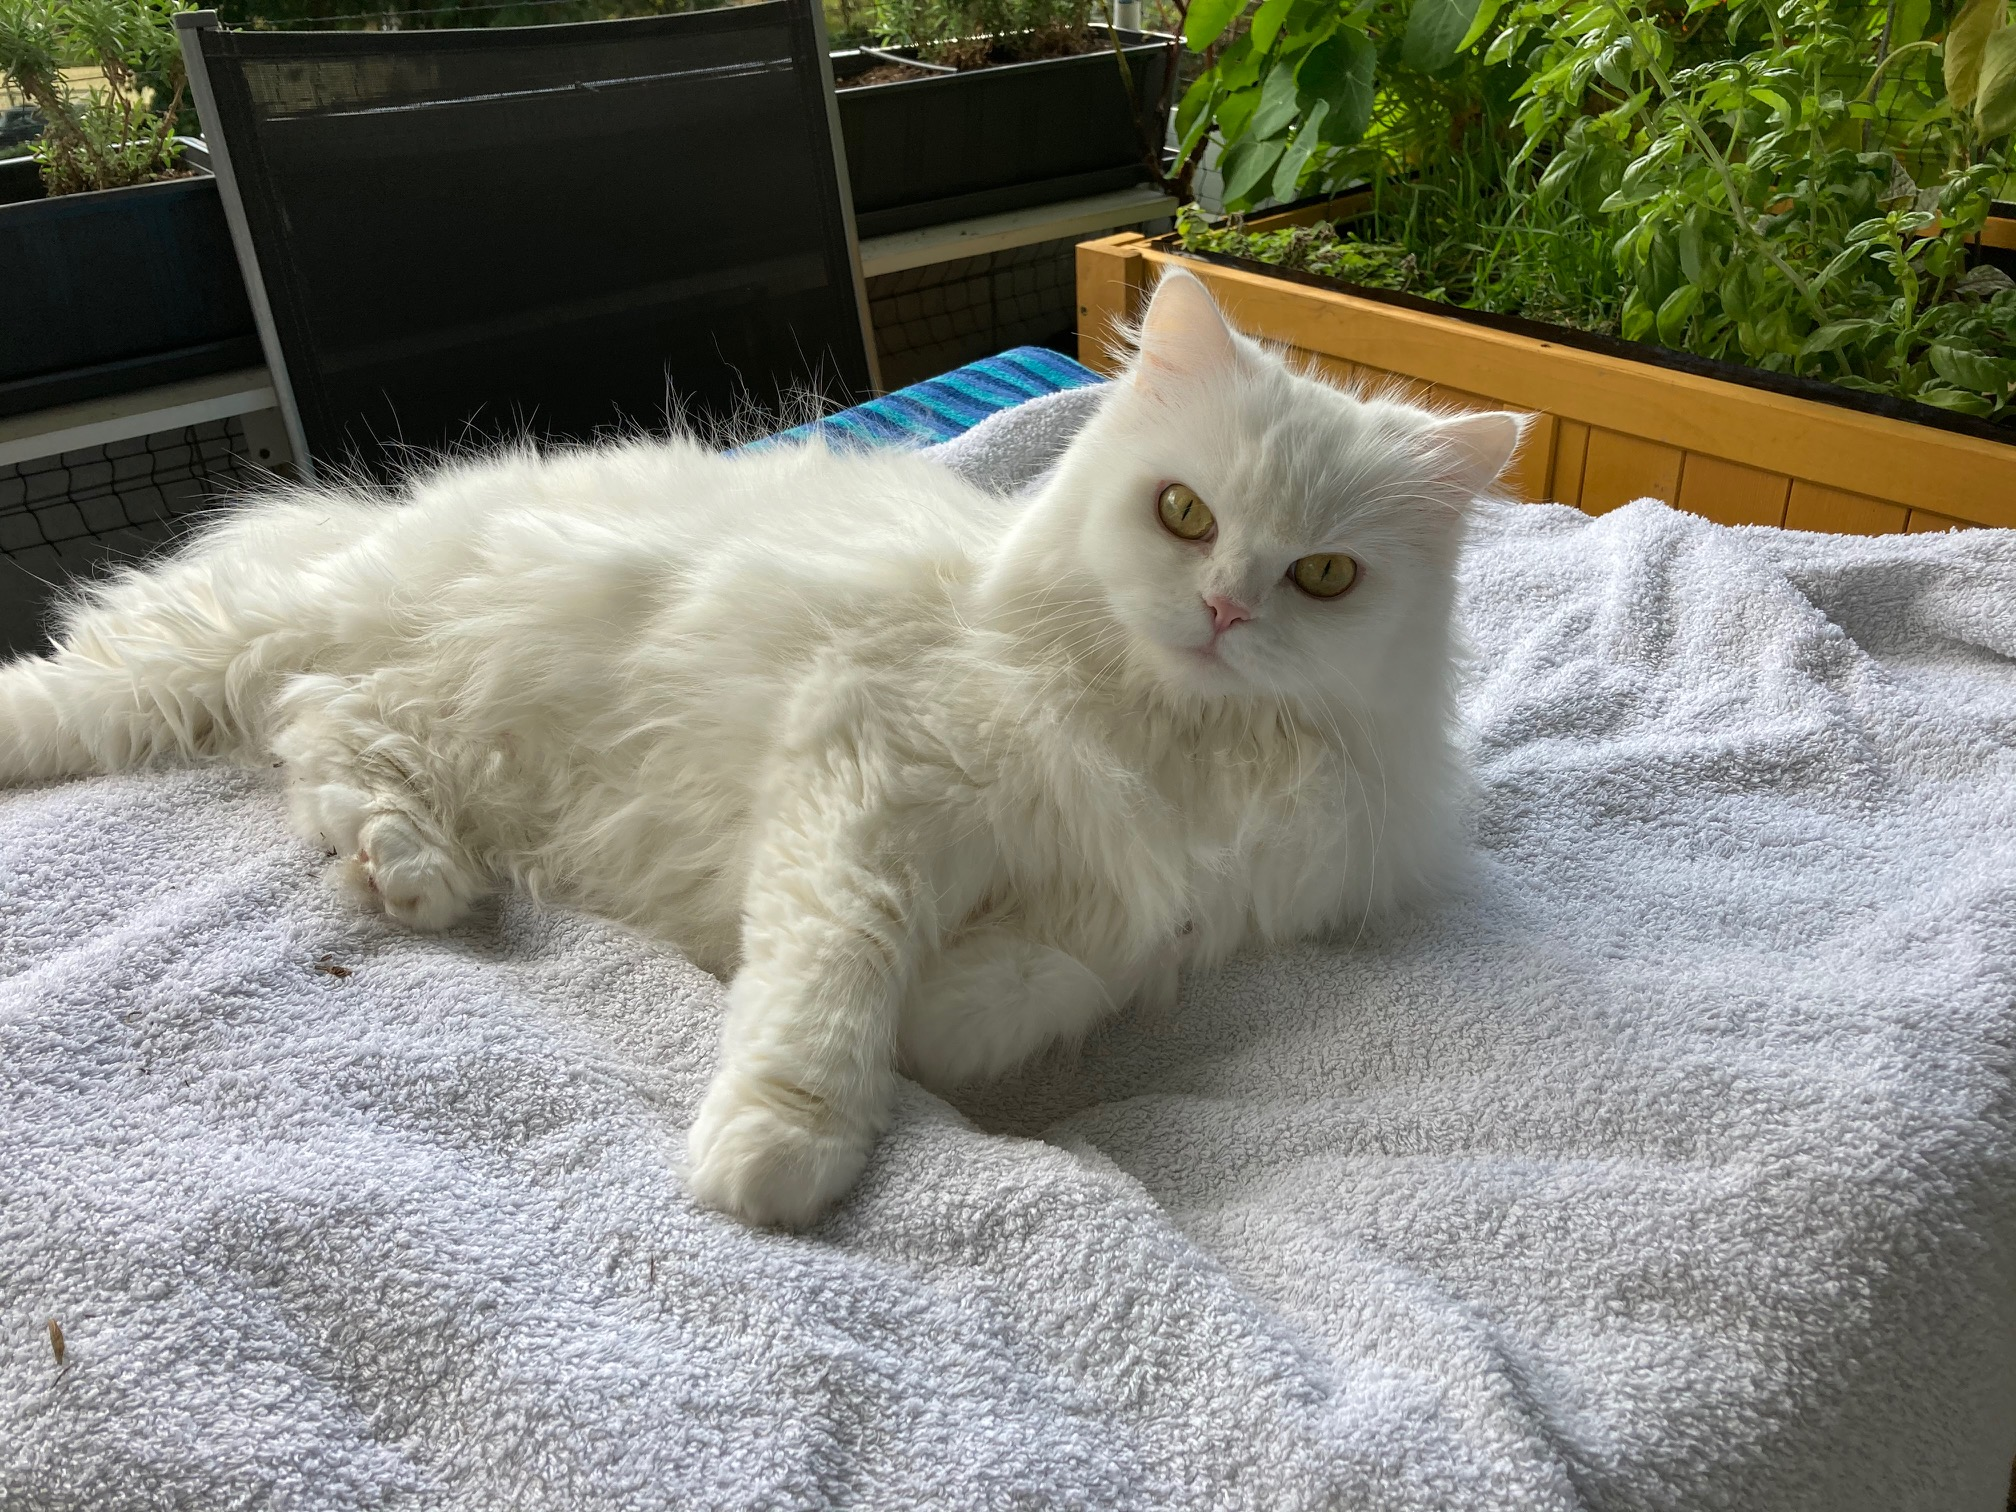
\includegraphics[width=0.49\textwidth]{Bilder/Katze1}}
	\subcaptionbox{Die selbe Katze \label{fig:cat2}}
	{
\includegraphics[width=0.49\textwidth]{Bilder/Katze2}}
	\caption{Zwei Katzenbilder}\label{fig:katzenbilder}
\end{figure}

Abbildung \ref{fig:cat1} auf Seite \pageref{fig:katzenbilder}

Abbildung \ref{fig:cat2} auf Seite \pageref{fig:katzenbilder}

Abbildung \ref{fig:katzenbilder} auf Seite \pageref{fig:katzenbilder}

\blindtext[2]
	
\end{document}

